% LTeX: enabled=false
\documentclass[english, he, bc, kiv, iso690alph]{fasthesis}
\usepackage{csquotes} % gets an annoying warning off of my face
\author{Radomír}{Kesl}{}{}
\supervisor{Doc. Ing. Roman Mouček, Ph.D.}
\title{Neural networks for processing recordings of brain electrical activity}
% TODO:
\assignment{zadani.pdf}
\signdate{31}{12}{2022}{V Nové Vsi u Nového Města na Moravě}
\addbibresource{references.bib}
\abstract{Text abstraktu v jazyce práce , tj. zde česky.}
{The abstract text in a secondary language, here in English.}
\keywords{šablona kvalifikační práce ,sazba ,DTP ,\LaTeX}
\acknowledgement{Text poděkování.}
% ENDTODO:
\begin{document}

\frontpages[tm]
\tableofcontents

% LTeX: enabled=true
% LTeX: language=en-GB

\chapter{Introduction}

Complex recordings of human brain electrical activity could help us uncover various secrets of the human brain and its disorders, as well as make progress towards brain-controlled computers.
Recording brain activity has recently been becoming increasingly common, especially the very needed large-scale experiments have started to emerge. Processing these however tends to be a complex task which usually requires a lot of time-costly manual work and prior knowledge of human staff and might be subjected to human bias. Using artificial intelligence for these purposes thus seems like a natural approach, and since the patterns of the brain tend to be complicated, the very advanced neural networks might be a great technique for tackling this problem.
This paper first discusses the background of this area from various perspectives then focuses on the state-of-the-art before presenting ideas for consecutive research. Finally, a subset of these ideas is chosen and implemented.
The purpose of this research is to help advance extraction of information from recordings of human brain electrical activity in order to make them more useful  for future medical research or for direct use in brain-computer interfaces.
This paper focuses on the application of neural networks on data from recordings of electrical activity of the human brain for processing and extracting key information.

% TODO: When done, adjust this to contain the specific form of the work

\chapter{Background}

In this chapter various concepts, important for the area of this work are briefly explained in the following order. First, electroencephalography is explained, secondly, brain-computer interfaces are discussed, after that motor imagery, a common task for brain-computer interfaces and electroencephalography, is introduced, before shortly mentioning data availability, one of the area's weaknesses. Lastly, deep learning classiffiers later used in the work are explained.

\section{Electroencephalography}

Electroencephalography (EEG) is possibly the most frequently used method of recording brain activity. It is conducted by planting electrodes on the scalp and making a record of the changing voltage (\cite{berger:eeg:29}, as cited by \cite{luck:erp:book}). This approach tends to be relatively convenient, as the required assets are not too costly, can be applied and removed non-invasively and even allow for user mobility~\cite{padfield:bci:19}.

The electrodes are usually placed according to the international 10-20 system, or alternatively with the newer 10-10 system. The numbers represent the percentage of the size of the skull, which is used to determine the space between the electrodes. In the 10-20 system it is 10\% and 20\% of the left-to-right and front-to-back direction, in the 10-10 system it is 10\% in both directions, resulting in more electrode placement options~\cite{acharya:channels:16}. The electrodes are marked with letters and numbers. The letters are as follows: A for ear lobe, T for temporal, F  for frontal, C for central, P for parietal and O for occipital. In the 10-10 system, letters can also come in pairs, denoting electrodes placed between two neighbouring areas. The numbers are odd for the left hemisphere and even for the right hemisphere, increasing with distance from the centre, which is marked with a 'z' instead.

\begin{figure}[h]
	\label{fig:channels}
	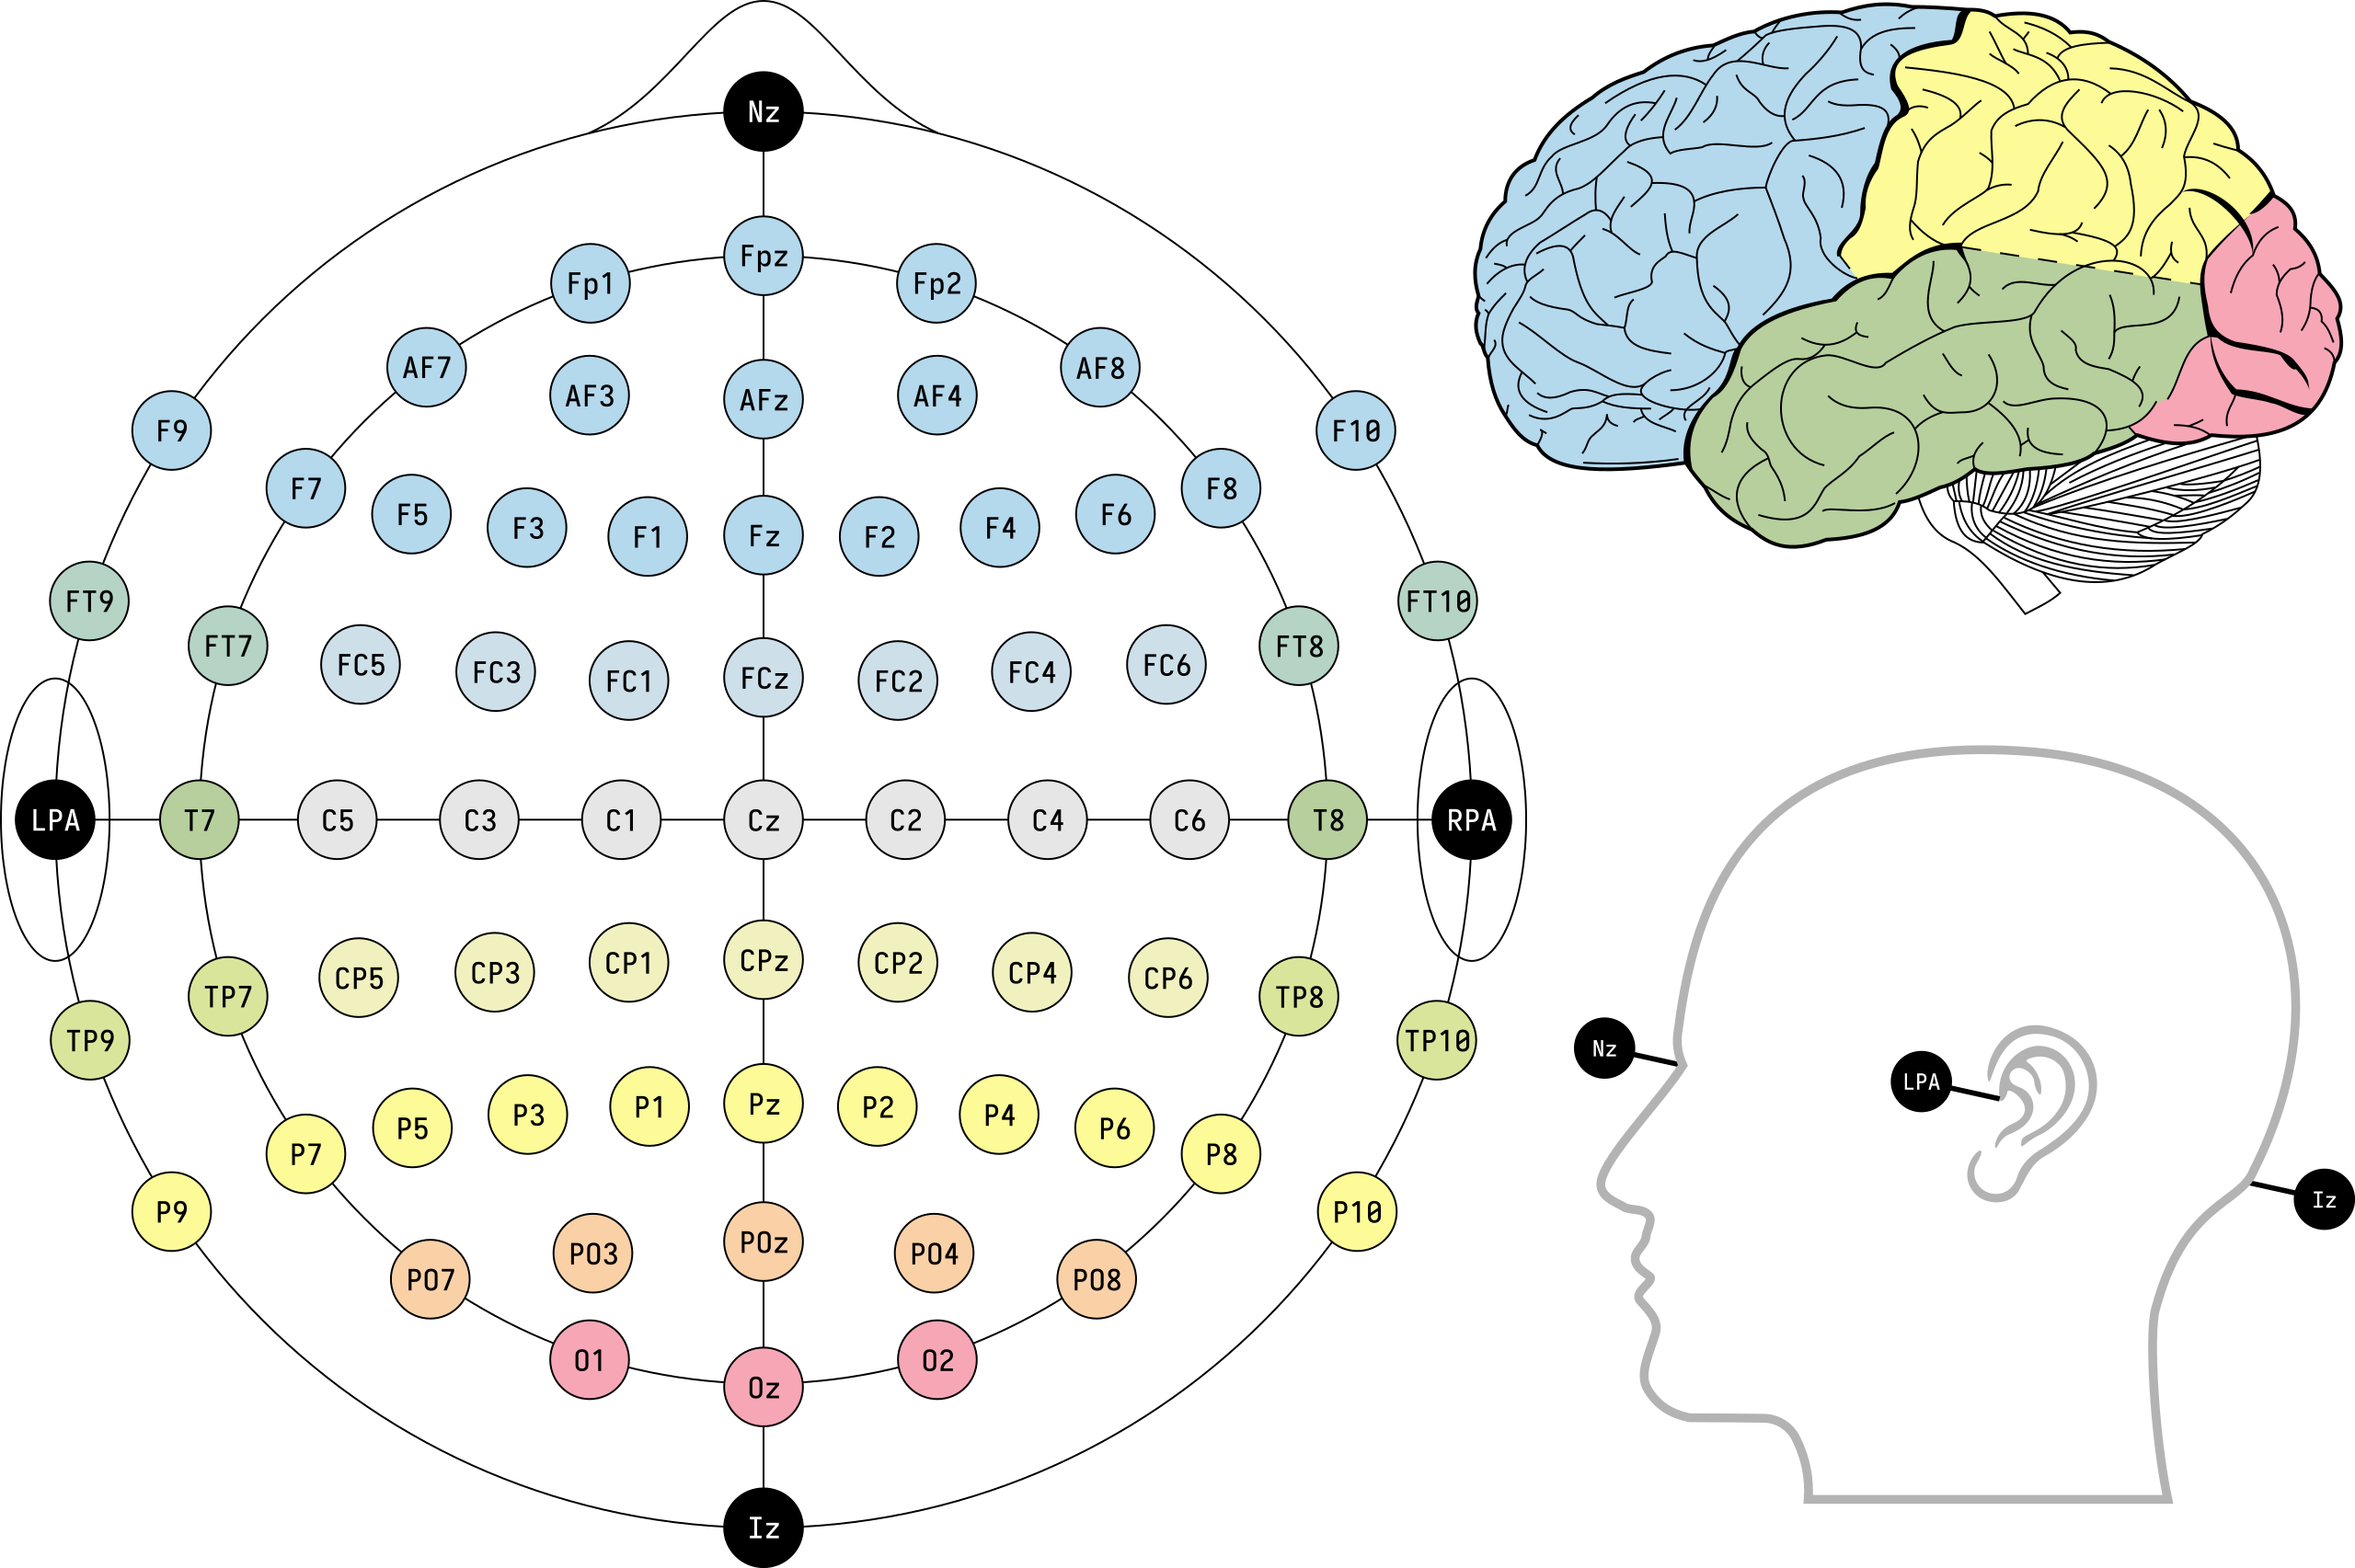
\includegraphics[width=\textwidth]{fig/channels.png}
	\caption{The 10-10 system of electrode placement. Source: \href{https://commons.wikimedia.org/wiki/File:EEG_10-10_system_with_additional_information.svg}{\textit{Wikimedia Commons}}.}
\end{figure}

One of the main advantages (along with the cost and convenience) of EEG is its great temporal resolution granted by the high speed of electric field propagation~\cite{roy:eeg:review:19}. On the other hand, the spatial resolution is often not great, which is caused by the tissues between the brain and the electrodes~\cite{roy:eeg:review:19, berezutskaya:ieeg:22}. A single electrode also obtains signals from several overlapping neural sources, leading to spatial correlation between the channels, making it difficult to isolate the desired information~\cite{roy:eeg:review:19, luck:erp:book}. In addition to that EEG also suffers noise from unrelated physiological signals, such as electromyogram from eye blinks~\cite{craik:dl:eeg:rev:19}.

It is worth noting that EEG can also be recorded intracranially (iEEG), possibly overcoming or at least reducing many of these issues. It is conducted by planting the electrodes directly on the brain tissue, which is obviously highly invasive and that tends to be a severe limitation, considering the risks and costs associated. There are, however, procedures that already involve the implantation process, such as localization of the source of epileptic seizures, or their treatment in drug-resistant patients~\cite{jobst:iEEG:20}. These provide a great opportunity to keep the records for other purposes as well~\cite{berezutskaya:ieeg:22}.

Lastly, one more disadvantage of EEG is high inter-subject variability caused by different physiology of subjects~\cite{roy:eeg:review:19}. This especially affects classification tasks that try to generalize over a large population. Intra-subject approach bypasses this problem, but introduces a new one --- the need for a large amount of data from each subject to train a unique classifier for them.

It appears that deep learning (DL) can be impactful in overcoming these limitations~\cite{roy:eeg:review:19}.

\section{Brain-computer Interface}
\label{sec:bci}

Using manual controls like buttons, joysticks or other physical movement is a serviceable but not very natural way of controlling assisting systems for the disabled~\cite{he:bci:legs:18}. This is only one of the areas, where brain-computer interface could be significantly beneficial~\cite{craik:dl:eeg:rev:19}.

As the name suggests, brain-computer interface (BCI), also referred to as brain-machine interface (BMI), could be defined as a system which allows direct communication between the human brain and a machine. However, controlling a BCI is typically challenging and requires extensive training, which still might be insufficient for some users~\cite{data:stieger:21}. The application of deep learning could help improve usability for users of varying proficiencies, making it easier to use for beginners and more precise for advanced users.

BCI technologies have a promising potential in various fields, such as prosthetics, rehabilitation and even entertainment.
In robotic prosthetics, BCIs could serve as an alternative to concurrent input methods, such as myoelectrics, which rely on relatively expensive technologies and are negatively affected by damage to the central nervous system~\cite{padfield:bci:19}. This also applies to wheelchair control and, in a sense, the control of a computer's cursor can fall in this category as well by providing even a seriously paralysed patient with numerous ways of interacting with the world.
In rehabilitation, robotic arms, exoskeletons and similar devices are often used to perform movements with the subjects' limbs in hopes of restoring the ability to do so on their own. In this practice, it is crucial for the subject to be imagining a movement of the limb and the device moving that limb in the imagined way. To achieve this, it is necessary to decode the imagination correctly, see section \ref{sec:mi}.
Another medical use of BCIs is affective computing, which is based on monitoring the subjects psychological state~\cite{padfield:bci:19}. This is a more passive approach, but the information is then used to for example adjust the subject's environment, so it can still be considered a BCI.
Finally, BCIs could be potentially used commercially in entertainment, for example gaming~\cite{padfield:bci:19}.

\section{Motor Imagery}
\label{sec:mi}

Motor imagery tasks seem to be among the most practical in BCI applications.
They rely on the subject imagining a movement of a part of their body without actually performing it~\cite{craik:dl:eeg:rev:19}.
The BCI then attempts to discern the imagined motion and passes the information to a connected system (assistant device, computer, \dots).

An interesting property of motor imagery is that it tends to have a similar effect on the brain as actually performing the movement~\cite{pfurtscheller:mi:01}. An important type of brain oscillation is the mu rhythm, also called the sensorimotor rhythm (SMR). It originates in the sensorimotor cortex and has frequencies in the range of 6-13 Hz. Its amplitude can become greatly suppressed in response to an internal or external event, such as sensory input, movement or mental imagery. This is often referred to as event-related desynchronization (ERD) and the usually following amplitude enhancement is called event-related synchronization (ERS). In SMR, ERD occurs with planning and initiating the execution of a movement and shortly after, ERS begins, returning to the original level within a few seconds. These activities seem to be present in the primary sensorimotor cortex with motor imagery similarly to actual motion performance, even though to a lesser extent~\cite{pfurtscheller:mi:01}. They can be most prominently measured on the C3, Cz and C4 electrodes, which are placed over the primary sensorimotor cortex, but also in the neighbouring ones, which you can see in figure \ref{fig:channels}.

\begin{figure}[h]
	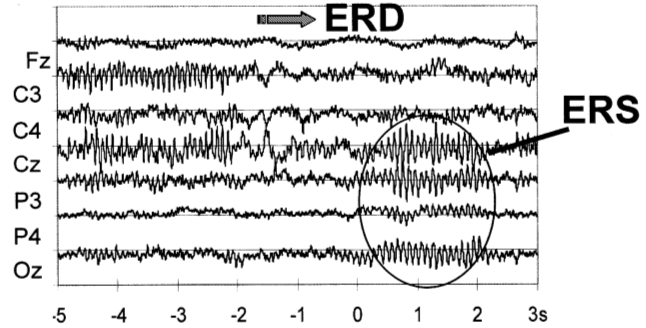
\includegraphics[width=\textwidth]{fig/erders.png}
	\caption{Ongoing EEG with right finger movement, $t=0s$ marks the start of movement. Note ERD prior to movement onset and ERS during movement \textcopyright 2001 IEEE,~\cite{pfurtscheller:mi:01}.}
\end{figure}

% 2) In the case of illustrations or tabular material, we require that the copyright line © [Year of original publication] IEEE appear prominently with each reprinted figure and/or table.

% One of the main advantages of this approach is that motor imagery (imagining a movement) tends to have a similar effect on the brain as actually performing the movement~\cite{pfurtscheller:mi:01} which can help verify the accuracy of the measurement, among other neurophysiological benefits~[\emph{ibid.}].
% That essentially means that we can record brain activity of subjects performing the movement and later compare it to the recordings from subjects imagining the movement to achieve better certainty that the data is valuable. If the data from motor imagery is nowhere near the data from performing movement, we can assume it is flawed (distracted subject, failed recording device, \dots) and exclude it from the final dataset.
% It also means that we have a better idea of what to look for in the patterns of brain activity and that we could potentially feed this information to neural networks --- learn them on data from performing movements instead of (or as well as) imagining them.

One advantage of motor imagery for BCI purposes is that it simulates natural ways in which humans control their movement. For example, imagining walking could be used to control assistant devices, like a wheelchair or a prosthetic leg, which would be a lot more natural than buttons and joysticks~\cite{he:bci:legs:18}. In addition, motor imagery can be exceptionally useful in rehabilitation, as discussed in section \ref{sec:bci}.

\section{Data Availability}

The lack of large, extensive datasets tends to be a problem while attempting to use neural networks on brain activity recordings. This is because complex classifiers, such as neural networks, while extremely precise with large amounts of data, tend to overfit easily in the case of insufficient data~\cite{domingos:ml:12}. This shortage seems to be mostly caused by the complexity of required experiments and the lack of appropriate subjects~\cite{he:da:21}. However, some studies that emerged recently appear reasonably extensive even for the use with these techniques.

Data augmentation (DA) --- a method of dealing with overfitting via generating additional data based on existing data --- tends to be a valuable tool in NN processing of brain activity recordings, because of the lack of complex datasets described earlier~\cite{he:da:21}. It carries some potential risks, such as reduced performance, but it usually succeeds in increasing accuracy of neural networks~[\emph{ibid.}].

% TODO: Maybe
% \section{Data Representation}

\section{Deep Learning Classification}

In this section, deep learning architectures that are later used in experiments are briefly described. That involves Convolutional Neural Networks, Long Short Term Memory Networks and Transformer Networks.

% TODO: CNN, LSTM, Transformer

\subsection{Convolutional Neural Network}

Convolutional Neural Network (CNN) is a type of neural network, originally mostly aimed at image classification. However, its main draw is its ability to extract patterns from the data, greatly reducing its dimensionality before classification, which applies to many types of data besides images. This reduction is achieved by only connecting neurons to a small part of the previous layer~\cite{oshea:cnn:15}. Because of its use in image processing, we often think about two-dimensional CNNs, applied to 2D data, but they can also be used for 3D data or, for our purposes, 1D data, such as the time series of EEG recordings.

The main components of Convolutional Neural Networks (CNNs) are convolutional layers and pooling layers. Fully connected layers, same as in standard multilayer perceptrons, are also needed to generate the final class scores for classification. Activation functions like ReLU are also usually used, and dropout layers can be added optionally to help prevent overfitting.

The convolutional layer is the core of CNNs. It applies small-sized filters, also called kernels to the input, convolving across it. That essentially means it slides through the input and computes scalar dot products between the kernel and each position in the input. The weights in the kernels, called activations, are what is actually learned by the model during training~\cite{oshea:cnn:15}. In a typical image classification task, such as the MNIST database of written digits, these can for example pick up on curves of the digits. Similarly, they are able to learn to recognize patterns in EEG data, such as the mu rhythm, or the event-related desynchronization and synchronization.

\begin{figure}[h]
	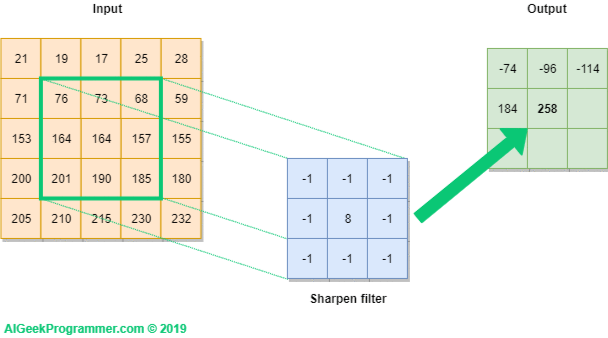
\includegraphics[width=\textwidth]{fig/conv.png}
	\caption{Convolution operation with a kernel of size 3x3 and step of 1. Step denotes by how many spaces the filter is moved every iteration. Source: \href{https://commons.wikimedia.org/wiki/File:CNN-filter-animation-1.gif}{\textit{Wikimedia Commons}}.}
\end{figure}

Pooling layers aim to further reduce the dimensionality by applying a function over a kernel-sized window of the input. The most common pooling function is max pooling, which outputs the maximum value in the window, but average pooling is common as well. While this operation generally preserves the most important information, it is still destructive in nature. For this reason, a kernel of size 2x2 is usually used. With a step of 2 (moving the kernel two spaces at a time) this results in a 75\% reduction of the input~\cite{oshea:cnn:15}.

\begin{figure}[ht]
	\centering
	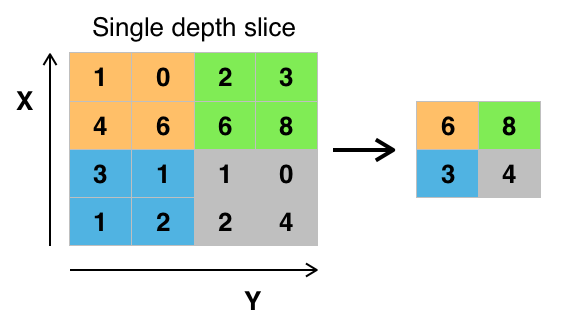
\includegraphics[width=0.75\textwidth]{fig/maxpool.png}
	\caption{Max pooling operation with a kernel of size 2x2 and step of 2. Source: \href{https://commons.wikimedia.org/wiki/File:Max_pooling.png}{\textit{Wikimedia Commons}}.}
\end{figure}

Overall CNNs' ability to extract patterns and reduce the complexity of models proves to be very useful in a variety of tasks, including EEG classification, where it can even overcome the noisiness~\cite{zhang:similar:20}.

\subsection{Long Short-Term Memory Network}

Recurrent Neural Networks (RNNs) are a type of neural network designed to process sequential data. They are able to remember previous inputs, which makes them suitable for time series data (such as EEG recordings). However, they tend to struggle with long-term dependencies, because of the vanishing and exploding gradient problem, a common issue with RNNs. This issue occurs during backpropagation, when the gradient is lower than 0 and the repeated multiplication leads to convergence towards 0 (vanishing) or higher than 1, converging towards infinity (exploding).

Long Short-Term Memory network is a type of RNN, designed to overcome this issue. It has a more complex structure, with a cell state, modifiable by gates, which are essentially neural networks themselves. The forget gate decides what information to forget (remove from the cell state), the input gate decides what information to add and with what weights, and the output gate decides what information to output. This structure allows the LSTM to remember information for a longer time, making it suitable for tasks with long-term dependencies~\cite{olah:lstm:15}.

\begin{figure}[ht]
	\centering
	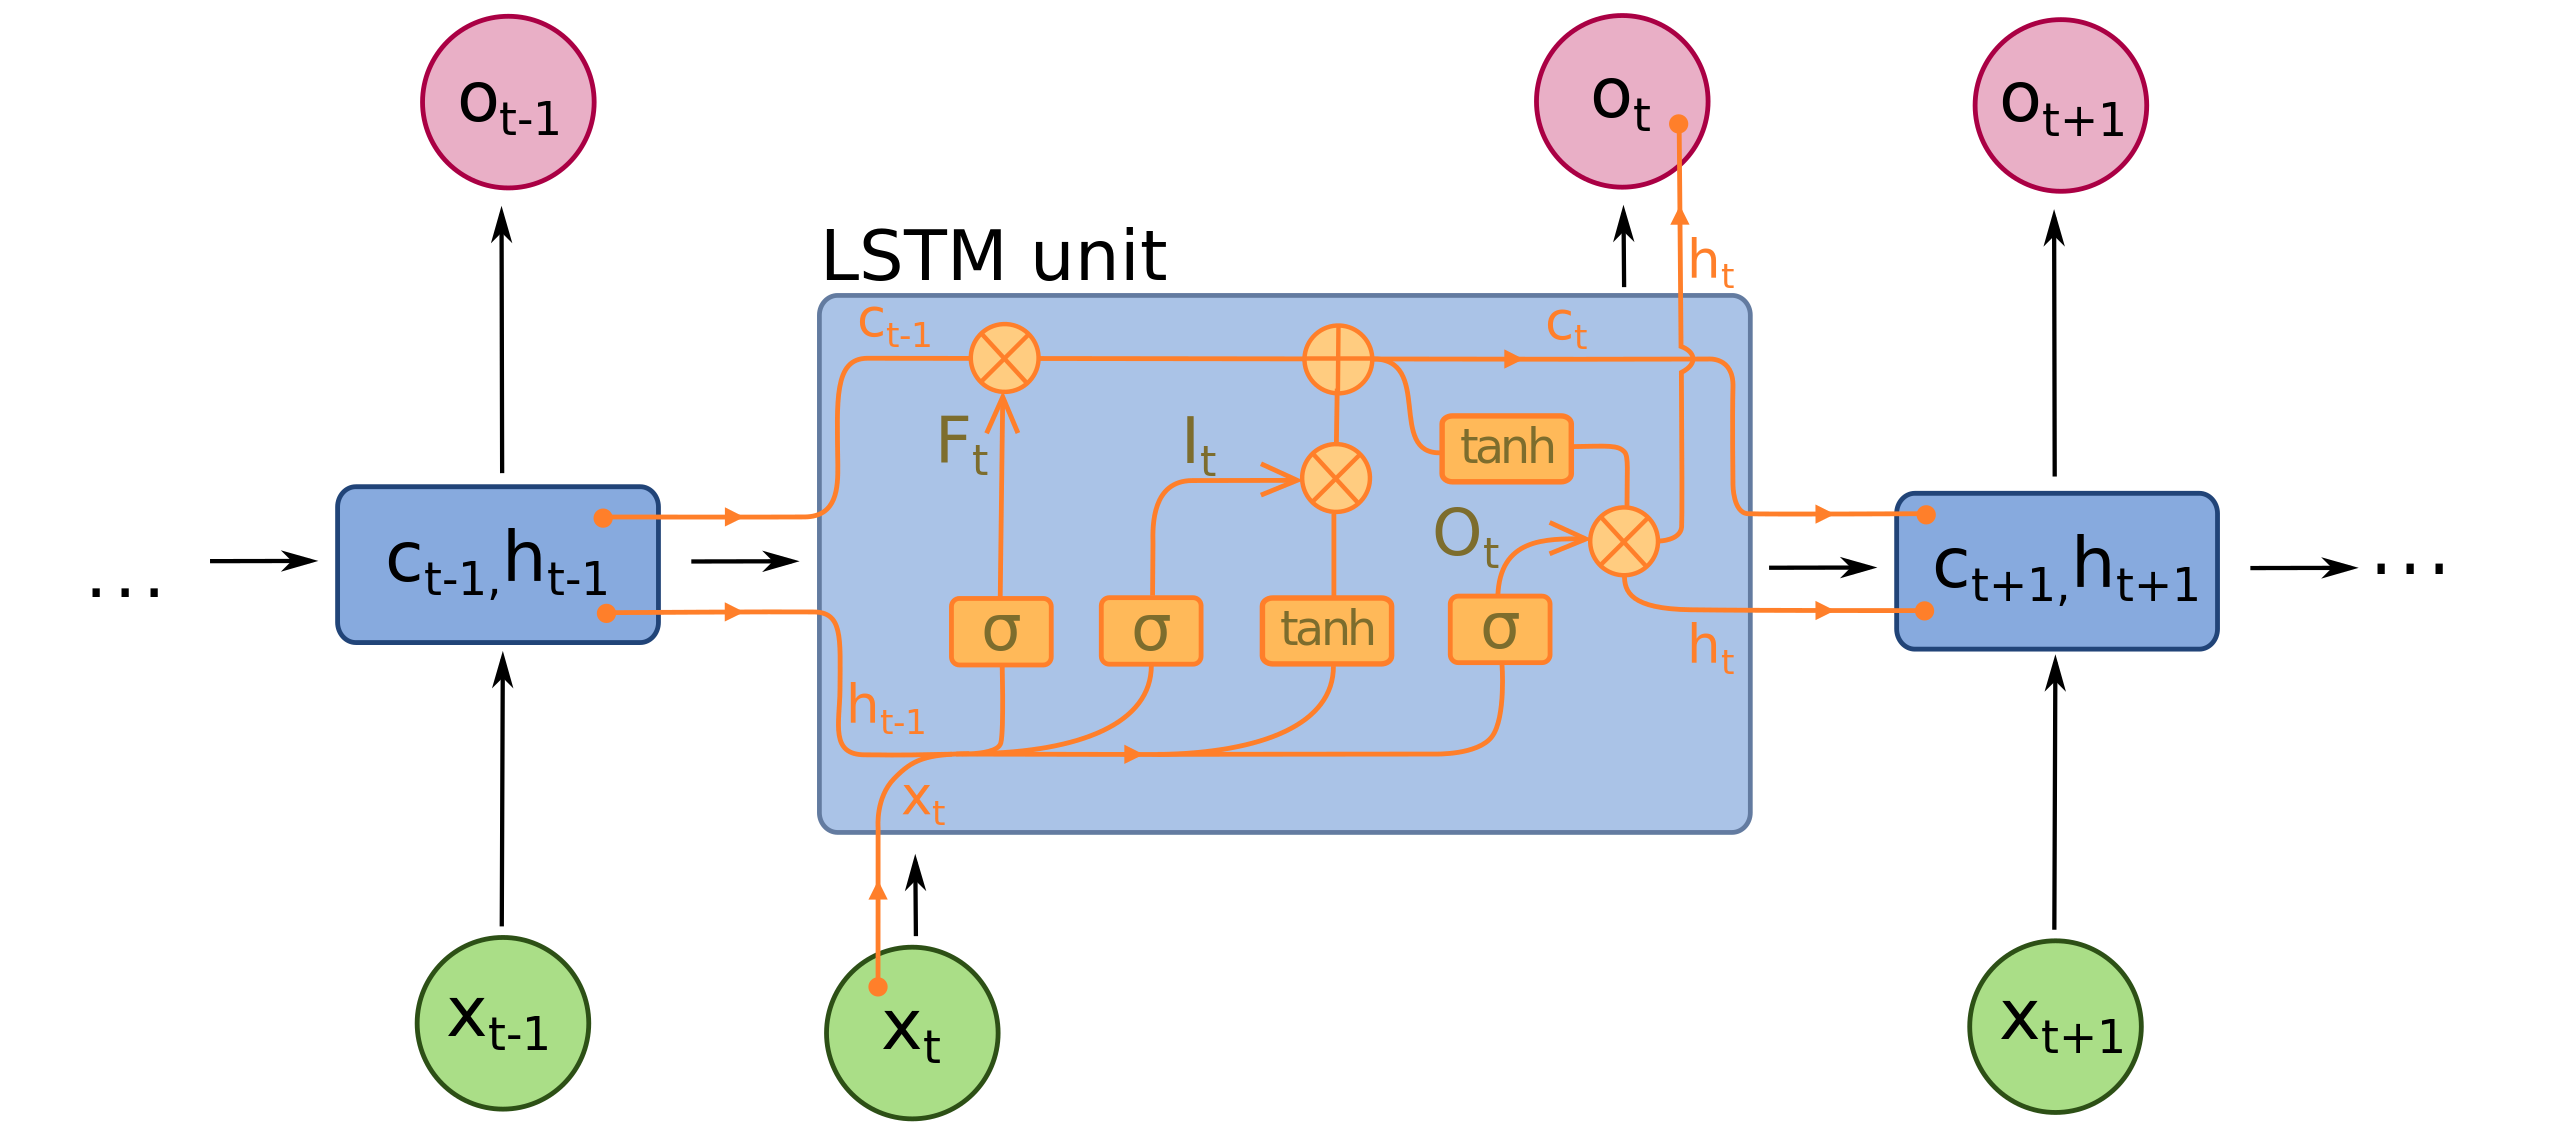
\includegraphics[width=\textwidth]{fig/lstm.png}
	\caption{LSTM unit. $F_t$ marks the forget gate, $I_t$ is the input gate and $O_t$ the output gate. $C$ symbolizes the cell state, $h$ the hidden state, $X$ marks the input, which gets concatenated with $h$ and $O$ marks the output, which is actually just a copy of $h$. Source: \href{https://commons.wikimedia.org/wiki/File:Long_Short-Term_Memory.svg}{\textit{Wikimedia Commons}}.}
\end{figure}

\chapter{State-of-the-art}

In the following chapter, some state-of-the-art research is presented and evaluated for the purposes of further examination. First new datasets of promising extensiveness are discussed and then examples of the application of modern deep learning systems on EEG data are shown.

\section{Datasets}

In this section, recent datasets are discussed in order to pick a good option for further experimenting. Each dataset has been assigned an alias (for convenience), as per table \ref{tab:aliases}. The examined sets have been recorded in table \ref{tab:datasets} and compared on metrics, such as size (amount of participants, trials and total recording time), metadata quality and availability. Further in this section a dataset is chosen and explained in detail. Note that this section is by no means meant to be a full review of the state-of-the-art datasets. It is a limited comparison with a goal of selecting a good set for our use. That means reasonably extensive, validated, equipped with metadata, accessible, and optimally already researched to an extent (other studies exist and can be used for comparison, but there is still space for further research).

The most of the comparison can be seen in table \ref{tab:datasets}. Note that trials and recording time are usually an approximation made by us or directly the authors of the dataset. The 'Citations' column contains the amount of times the data paper was cited according to Web of Science at the time of writing this. The 'Metadata' column shows the quality of the metadata, attached to the dataset, where 'Sufficient' means at least gender, age and laterality; 'Insufficient' means anything less than that; and 'Extensive' means substantially more than that.
Based on our findings, the Stieger-62 dataset was chosen for further experimentation. The main reason is its size, which beats all the listed competition (and likely most of the unlisted as well) and while the Dreyer-87 dataset has a greater number of participants, the amount of trials and recording time in Stieger-62 is far superior, and we consider that more important. This dataset also fulfils all other requirements (validation, accessibility, \dots) and has a reasonable amount of citations. For those reasons it will be examined more closely and likely chosen for our experiments. If new issues appear about it, the Dreyer-87 dataset will be considered.

\begin{table}
	\centering
	\begin{tabular}{@{}p{0.15\textwidth}p{0.6\textwidth}p{0.15\textwidth}@{}}
		\toprule
		\textbf{Alias}        & \textbf{Article name}                                                                                    & \textbf{Citation}       \\
		\midrule
		Dreyer-87             & A large EEG database with users’ profile information for motor imagery brain-computer interface research & \cite{data:dreyer:23}   \\
		Ma-25                 & A large EEG dataset for studying cross-session variability in motor imagery brain-computer interface     & \cite{data:ma:22}       \\
		Peterson-10           & A motor imagery vs. rest dataset with low-cost consumer grade EEG hardware                               & \cite{data:peterson:22} \\
		Stieger-62            & Continuous sensorimotor rhythm based brain computer interface learning
		in a large population & \cite{data:stieger:21}                                                                                                             \\
		\bottomrule
	\end{tabular}
	\caption{Aliases of compared datasets.}
	\label{tab:aliases}
\end{table}

\begin{table}
	\centering
	\resizebox{\textwidth}{!}{
		\begin{tabular}{@{}*{9}{l}@{}}
			\toprule
			\textbf{Dataset} & \textbf{Participants} & \textbf{Trials} & \textbf{Recording time} & \textbf{Citations} & \textbf{Metadata} & \textbf{Validation} & \textbf{Availability} & \textbf{Licence} \\
			\midrule
			Dreyer-87        & 87                    & 20800           & 70 hours                & 0                  & Extensive         & Present             & Open Access           & CC BY 4.0        \\
			Ma-25            & 25                    & 12500           & 26 hours                & 6                  & Insufficient      & Present             & Open Access           & CC BY 4.0        \\
			Peterson-10      & 10                    & 1650            & 15 hours                & 1                  & Sufficient        & Missing             & Open Access           & CC0              \\
			Stieger-62       & 62                    & 250000          & 600 hours               & 15                 & Extensive         & Present             & Open Access           & CC BY 4.0        \\
			\bottomrule
		\end{tabular}
	}
	\caption{Comparison of recent datasets.}
	\label{tab:datasets}
\end{table}

% TODO: Review and edit

\subsection{Stieger-62 Dataset}
\label{subsec:stieger-62}

The Human EEG Dataset for Brain-Computer Interface and Meditation, collected by Stieger et al.~\cite{data:stieger:21} appears to be among the best in class with more than 250000 trials from 62 subjects, collected over 7--11 sessions.
The task in these experiments was moving a cursor via imagining hand movement. The subject was supposed to imagine opening and closing their left or right hand to move the cursor in the respective direction, opening and closing both hands at once to move the cursor up and clearing their mind to move the cursor down. Third of the trials was limited to up-down movement, third to left-right movement and the rest in both dimensions.
The 2D movement is a relatively uniquely complex task among BCI experiments.
Another important point is that one of the purposes of the study was to examine the evolving proficiency as the subject underwent successive sessions which could serve potential DL analysis.
Some subjects also received training in mindfulness and meditation, as examination of the effects of this training on BCI proficiency was among the main interests of the study~\cite{stieger:mindfulness:20}. It is worth noting that this dataset suffers a major gender imbalance with 49 out of the 62 subjects being female. This might be the result of the aforementioned training in mindfulness and meditation being offered as a reward for participating in the study~\cite{data:stieger:21}.

This, together with other metadata, which is provided in great measure for the dataset, could be used to conduct various experiments in order to improve accuracy of the BCI using neural networks.
The data was already classified online, using an autoregressive model with the maximum entropy method to allow the users to control the cursor and thus be able to include the subjects' response to the visual feedback in the data, therefore it seems natural to attempt to use a DL based method and compare the outcomes, possibly helping the subjects achieve better results.

\section{Deep Learning on EEG Studies}

This section provides examples of recent studies in a similar scope as this work, which means mostly using deep learning on EEG data.

\subsection{On the Deep Learning Models for EEG-Based Brain-Computer Interface Using Motor Imagery}

This study by Zhu et al.~\cite{zhu:dl:bci:mi:22}, uses the Stieger-62 dataset, comparing state-of-the-art DL systems, conducting a within-subject analysis, as well as a cross-subject analysis. Only a limited subset of the dataset was used by the authors in order to allow comparability to another dataset. Specifically, only one of three tasks was used --- moving the cursor from left to right, up-down movement and 2D movement were omitted. Additionally, only the first three sessions from each user were included.
The following algorithms were used: EEGNet (CNN), Deep and Shallow ConvNet, Multi-Branch 3D CNN (CNN with 3D tensor input, arranged by spatial position on the scalp) and ParaAtt (Parallel Self-Attention Network). In the within-subject analysis, a model was built for each subject, using recordings from the first two sessions for training (20\% of that for validation) and data from the third session for testing. All the algorithms have outperformed the maximum entropy model, used for online evaluation in the within-subject analysis. However, only EEGNet surpassed the online evaluation in a statistically significant way, achieving accuracy of $75.47 \pm 10.8\%$, while online achieved $68.10 \pm 12.6\%$.\@
For the cross-subject analysis, a model was also built for each subject, only this time using the first three sessions from that one subject as the test set  and the first three sessions of the remaining subjects as the training set (again, 20\% for validation). According to the authors of the study, EEGNet performed the best again (better than all the other models in a statistically significant way), but they do not provide the specific numbers.
This appears to be the only extensive study, conducted on the Stieger-62 dataset so far (and reasonably accessible to us) at the time of writing this, which leaves a decent amount of space for further studies while providing a possibility of comparison.

\subsection{Applying Deep Learning for Decoding of EEG and BFV about Ischemic Stroke Patients and Visualization}

This paper by Zhang and Wu~\cite{zhang:similar:20} aims to detect the Modified Rankin Scale (mRS)\footnote{Modified Rankin Scale is a scale for measuring the severity of disability of stroke patients. It ranges from 0 for no symptoms to 6 for death.} of ischemic stroke patients using EEG and blood flow velocity (BFV) data. They only use a small dataset of 15 subjects, 14 of which are ischemic stroke patients and one is healthy. They conducted experiments using a CNN, an LSTM and a CNN-LSTM hybrid. The hybrid achieved the best results with an accuracy of 99.68\%, which is a very promising result. It should be noted that on a patient in the state of dying the classifier failed, likely due to insufficient representation of that class in the dataset, but another reason might be a more chaotic behaviour of the brain in that state. As a result, the authors warn that this architecture might not be suitable for applications with rapidly changing signals.

\chapter{Analysis}

Ideas for future research in the application of neural networks on brain activity data, mostly based on the unique features of the Stieger-62 dataset, are proposed in this chapter. Some of these will be selected for the final application. First, new approaches on using specific data for training NNs in BCIs are suggested, then a more effective approach to storing data for experiments is discussed.

\section{Training on Data from Proficient Users}

According to Stieger et al.~\cite{data:stieger:21,stieger:mindfulness:20} users can improve in BCI proficiency via training. The question is: Could learning on recordings from these advanced users produce better classifiers than simply using all the available data? And would these be effective for any user or only those of comparable abilities?

This issue appears to be worth investigating via experimentation and the Med-62 dataset~\cite{data:stieger:21} could be very useful for that. Training neural networks on this whole dataset and comparing the results to the same classifiers, learned on the later sessions only, could be  attempted. Also adding data augmentation to both of the experiments might produce interesting results --- the dataset is large enough, so that such a tool does not seem necessary, but it could still improve the accuracy, especially if only a part of the dataset is used.

Additionally, similar experiments could be performed with focus on users who received training in meditation instead of or in addition to using the later sessions.

\section{Metadata Specific Training}
\label{sec:metadata:specific}

Another, slightly similar, approach that could be attempted is trying to find a classifier which would best work for a specific group of subjects based on a shared quality, such as gender, age and task-specific subject traits (such as dominant hand in the case of motor imagery). This could be done by training an entire subject-specific classifier which in case of long term used systems, such as BCI-operated assistant devices, would probably still be worth the extra work, or by pre-training a general classifier and then adding specializations for each user.

This approach seems to require a large amount of data equipped with profound metadata and once again, the Med-62 dataset~\cite{data:stieger:21} appears appropriate for that. In addition, as using subsets of datasets reduces the volume of the data significantly, data augmentation would likely be a worthwhile tool for these methods.

\section{Unified and Efficient Approach to Data}

Speaking from a completely different perspective, it does seem that this area of research could benefit from a more unified approach to some procedures, such as data recording and especially storage. A system where the data is in a single binary file could be designed. All the metadata could be in an external database or a similar system which would provide very fast access to any subset of the dataset, based on the metadata --- basically via simple queries.

A system like this could for example simplify the experiment procedure and increase the performance of metadata specific training discussed above. However, unification of the storage would probably be just useful in general, it could lead to better comparability between studies and much more complex and useful benchmarks.

\chapter{Implementation}

In this chapter, the specifics of the experiment, that was conducted in this work are explained. Most of these came about from an agreement with the thesis advisor or were the result of "metaexperimentation" during the development. By metaexperimentation, manual testing of models with different architectures and hyperparameters built upon a small subset of the dataset, as well as with different preprocessing approaches, is meant. Note that all the parameters and hyperparameters that were chosen in this way and used in the experiments are set as defaults in the associated code.

The Stieger-62 dataset was eventually selected for the experiments and the general decided direction was to focus on models for a specific group of subjects, based on shared metadata.

The resulting application has been split into two independently working parts. The first part is a data processing tool, the purpose of which is to load the data, as provided by the dataset authors, process it and save it in a format, which is then directly digestible by the models. This includes filtering the data, based on subject metadata, artefact removal and more. The second part is capable of training and testing the models themselves. Its output is a trained model for potential future use and a report on the model's performance.

Both parts were built in the Python programming language, using the following libraries:

\paragraph{NumPy:} A library providing high-level mathematical operations, mostly for working with n-dimensional arrays. In this work it is used during the loading process, for reducing the data in the desired way and artefact removal.

\paragraph{SciPy:} A library providing mostly tools for scientific computing. Here it is only used for loading \texttt{MATLAB}-formatted data into Python's structures (dictionaries and \texttt{NumPy} arrays).

\paragraph{PyTorch:} A mostly deep learning-focused library, providing tools for building and training neural networks. It has a relatively low level of abstraction, allowing for high control over the models. \texttt{PyTorch} mostly works with tensors, which are similar to \texttt{NumPy} arrays, but can for example be moved to an accelerator (such as a GPU) for faster computation. It is mainly used to create the architecture of the models, but the loader also saves the data as \texttt{PyTorch} tensors.

\paragraph{Scikit-learn:} A library providing tools for machine learning. It is only used for creating folds for k-fold cross-validation.

\paragraph{PyTorch Lightning:} A library built on top of \texttt{PyTorch}, providing a higher level of abstraction, sacrificing control in order to reduce boilerplate code and increase readability. It is used for the training and testing processes.

\paragraph{TorchMetrics:} A library providing high-level tools for gathering metrics for \texttt{PyTorch} and \texttt{PyTorch Lightning} models. It is used to gather metrics while testing the models.

\section{Data Loading and Preprocessing}

Most of this work is done by the \texttt{Loader} class in the \texttt{loader.py} file and its method \texttt{load\_dir}, which when pointed to a directory will load all the \texttt{.mat} files in it, process them and return the data in the form of \texttt{PyTorch}'s \texttt{TensorDataset} as well as information about the data. Upon construction, the \texttt{Loader} is passed a group of parameters, defining what part of the dataset it will specifically load. These parameters are explained throughout this chapter. In addition to that, a \texttt{LoadSuite} class is provided (in \texttt{load\_suite.py}), which adds the ability to run multiple loads in succession, allowing to load multiple subsets of the dataset and save them in a structured way, along with the metadata.

\subsection{Data Format}

As stated previously, the Stieger-62 dataset, described in \ref{subsec:stieger-62} is used. It was recorded from 62 subjects of age 18--63, 49 of which are female. Seven or eleven sessions were recorded with each user, consisting of 450 trials each, 150 per task. The tasks were moving a cursor up and down, left and right and in both dimensions. The data was recorded using a 64-channel EEG cap, with a sampling rate of 1000 Hz.

The set is provided as a collection of \texttt{MATLAB .mat} files, each coming from a single recording session from a single subject, resulting in 598 files total. Each file contains the raw data, trial-specific metadata, subject-specific metadata and channel information.
The data is stored separately for each trial. Along with it, the duration of each trial is stored, as it differs between trials. Additionally, the cursor position at every recording moment (millisecond) is stored, as well as the recording rate, though the latter is constant for all trials.
The trial-specific metadata includes the task, the target, the result (whether the trial was successful online) and more.
The subject-specific metadata includes the age, gender, laterality, but also whether the subject considers themselves an athlete, has a hobby that requires fine motor skills and so on.

For more specifics, see \href{https://figshare.com/articles/dataset/Human_EEG_Dataset_for_Brain-Computer_Interface_and_Meditation/13123148?file=25302482}{\textit{the repository}} or the related data paper~\cite{data:stieger:21}.

\subsection{File selection}

As stated previously, the main goal of the experiment would be to train intra-subject models, but based on shared metadata. Since the dataset is provided in separate files by session, we can process them one by one, only adding to the dataset trials from the subjects that meet our criteria, avoiding the need to hold more than one \texttt{.mat} file in memory at a time (we still need to hold all the accepted trials in order to be able to save them as \texttt{PyTorch} tensors). This is the first step of the data loading process.

The first tool the \texttt{Loader} class provides is the ability to hand-pick specific users or sessions by number. These can be provided to the \texttt{Loader} as constructor arguments in the form of lists. This can be useful for example for creating small datasets for testing purposes, or for selecting only the later sessions, where users are expected to be more proficient. It also speeds up the loading process, because this information is encoded in file names, so the \texttt{Loader} does not need to actually load the \texttt{.mat} files, which were not selected.

The main idea, however, is accepting only trials from subjects who match a specific set of criteria. For this reason, the \texttt{load\_dir} method always first (after loading the file) checks, whether the subject specific metadata matches the criteria and if not, immediately moves on to the next file. The criteria are passed to the \texttt{Loader} as a \texttt{SubjectSpec} object, which is a dataclass, where the required criteria can be specified. The options correspond to subject-specific metadata fields in the dataset and can be seen in code sample \ref{lst:subjectspec}. This class implements a \texttt{passes} method, which checks a dictionary of subject metadata (directly extracted from the loaded file by the \texttt{load\_dir} method) against the criteria it represents.

\begin{code}{Python}{Header of the SubjectSpec dataclass. All of these fields can be set in the constructor. If a field is set to \texttt{None}, this criterion will not be checked. The "\texttt{range}" criteria are inclusive on the lower end and exclusive on the upper end.\label{lst:subjectspec}}
	@dataclass
	class SubjectSpec:
	gender: Optional[Literal["M", "F"]] = None
	age_range: Optional[Tuple[int, int]] = None
	handedness: Optional[Literal["R", "L"]] = None
	mbsr: Optional[bool] = None
	meditation_hours_range: Optional[Tuple[float, float]] = None
	instrument: Optional[List[Literal["Y", "U", "N"]]] = None
	athlete: Optional[List[Literal["Y", "U", "N"]]] = None
	handsport: Optional[List[Literal["Y", "U", "N"]]] = None
	hobby: Optional[List[Literal["Y", "U", "N"]]] = None
\end{code}

\subsection{Preprocessing}


% \appendix
% \chapter{Appendix A}

\backmatter
\printbibliography
\backpage

\end{document}


